%%%%%%%%%%%%%%%%%%%%%%%%%%%%%%%%%%%%%%%%%%%%%%%%%%%%%%%%%%%%%%%%%%%%%%%%
%                                                                      %
%     File: Thesis_Results.tex                                         %
%     Tex Master: Thesis.tex                                           %
%                                                                      %
%     Author: Andre C. Marta                                           %
%     Last modified :  2 Jul 2015                                      %
%                                                                      %
%%%%%%%%%%%%%%%%%%%%%%%%%%%%%%%%%%%%%%%%%%%%%%%%%%%%%%%%%%%%%%%%%%%%%%%%

\chapter{Results}
\label{chapter:results}

This chapter will be presenting the results in the behaviour of the aircraft for the different solutions proposed to control and stabilise it. Once the goal for the results of this chapter is properly established, the first step will be to validate the model that was implemented. This will be done by controlling the aircraft into cruise conditions using the baseline feedback linearisation error. The effects of disturbances and inversion errors will then be studied regarding their effects in aircraft dynamics. The next step will be to achieve the goal of this thesis and demonstrate the effects of an on-line neural network in reducing the tracking error in the presence of these disturbances. Finally, from the adaptive controller, including the neural network, the guiding law described in chapter \ref{chapter:implementation} in \ref{eq:guidance_law} will be added to follow a given trajectory.


%%%%%%%%%%%%%%%%%%%%%%%%%%%%%%%%%%%%%%%%%%%%%%%%%%%%%%%%%%%%%%%%%%%%%%%%
\section{Model Validation}
\label{section:results/validation}

The goal in this section will be to validate the behaviour of the model in cruise conditions. Assuming cruise conditions comes that

\begin{gather}
	T=D\\
	W=L\\
	L'=M=N=0
\label{eq:cruise_cond}
\end{gather}
In order to verify the model described so far, the required thrust to have cruise conditions will be computed for a given plausible value of $\alpha$. From this point the airspeed of the aircraft can also be computed. The graph of $C_L$ versus alpha was also obtained from its respective neural network, given by \ref{fig:cl_alpha}
\begin{figure}[!htb]
  \centering
  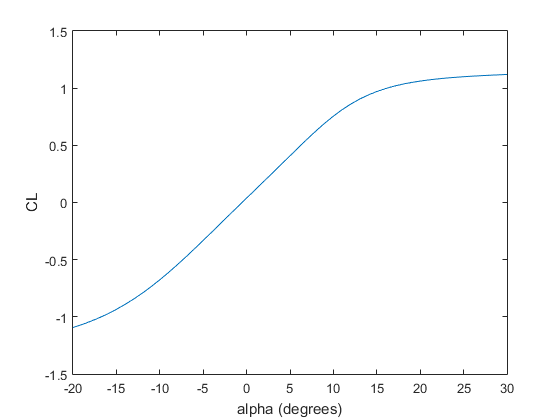
\includegraphics[width=0.75\textwidth]{Figures/CL_alpha.png}
  \caption[$C_L$ versus $\alpha$ graph]{$C_L$ versus $\alpha$ graph from Neural Network}
  \label{fig:cl_alpha}
\end{figure}
From the cruise conditions \ref{eq:cruise_cond}, knowing that $L=\dfrac{1}{2}\rho S V^2 C_L$, solving for the airspeed V comes that

\begin{equation}
V=\sqrt{\dfrac{2mg}{\rho S C_L}}
\label{eq:cruise_speed}
\end{equation}
The required thrust can also be computed from both \ref{eq:cruise_cond}, \ref{eq:cruise_speed} and \ref{eq:cd_cl}, knowing the $C_L$ for a given angle of attack. Proposing some values of $\alpha$, the following results are obtained

\begin{table}[htbp]
  \centering
  \caption{Required cruise conditions for different values of $\alpha$}
    \begin{tabular}{ccccc}
    \toprule
    $\alpha (^o)$ & $C_D$ & $C_L$ & $V (ms^{-1})$ & $T (N)$ \\
    \midrule
    0     & 0.017677131 & 0.0387 & 707.4010791 & 224047.3585 \\
    2     & 0.019379779 & 0.1859 & 322.7613368 & 51133.84325 \\
    4     & 0.023345134 & 0.334 & 240.7952785 & 34283.79709 \\
    6     & 0.029604436 & 0.4828 & 200.279994 & 30076.58604 \\
    \bottomrule

    \end{tabular}%
  \label{tab:cruise_cond}%
\end{table}%

From these values, to test both the model (as well as the methods used to simulate the dynamics of the aircraft, including the coefficients neural networks)and the feedback linearisation controller, the following reference values $V_a^d=200 ms^{-1}$, $\gamma^d = 0 rad$ and $\psi^d=0 rad$ were used in an attempt to simulate cruise conditions. From there the values of thrust and angle of attack were computed and  compared to the theoretical values of table \ref{tab:cruise_cond}. 
Following these constant reference values the results obtained were

\begin{figure}
\centering
\begin{minipage}{0.49\textwidth}
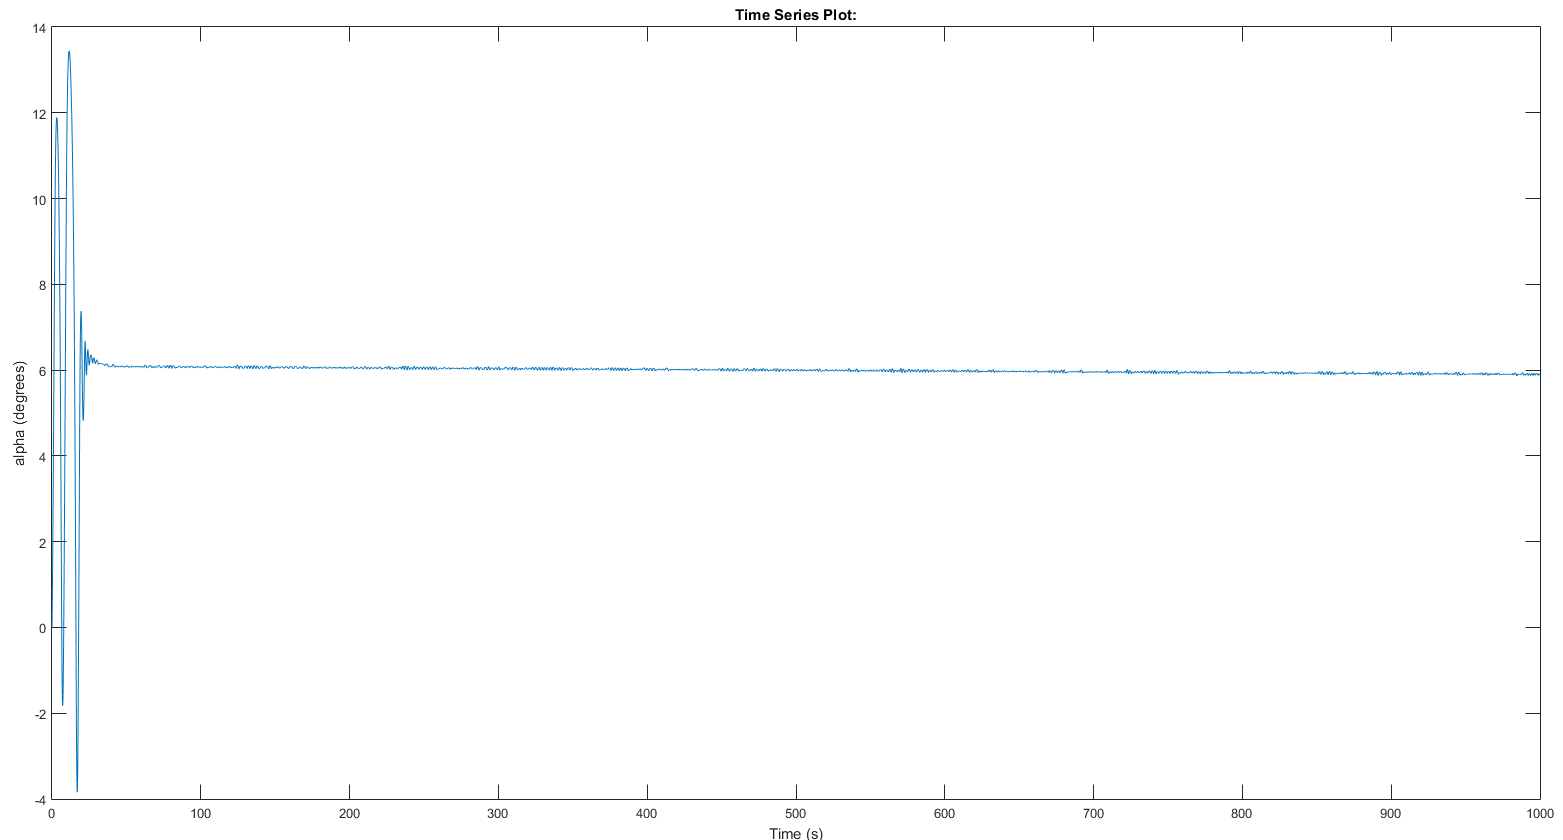
\includegraphics[width=\textwidth]{Figures/Results/aoa_check.PNG}
\end{minipage}
\begin{minipage}{0.49\textwidth}
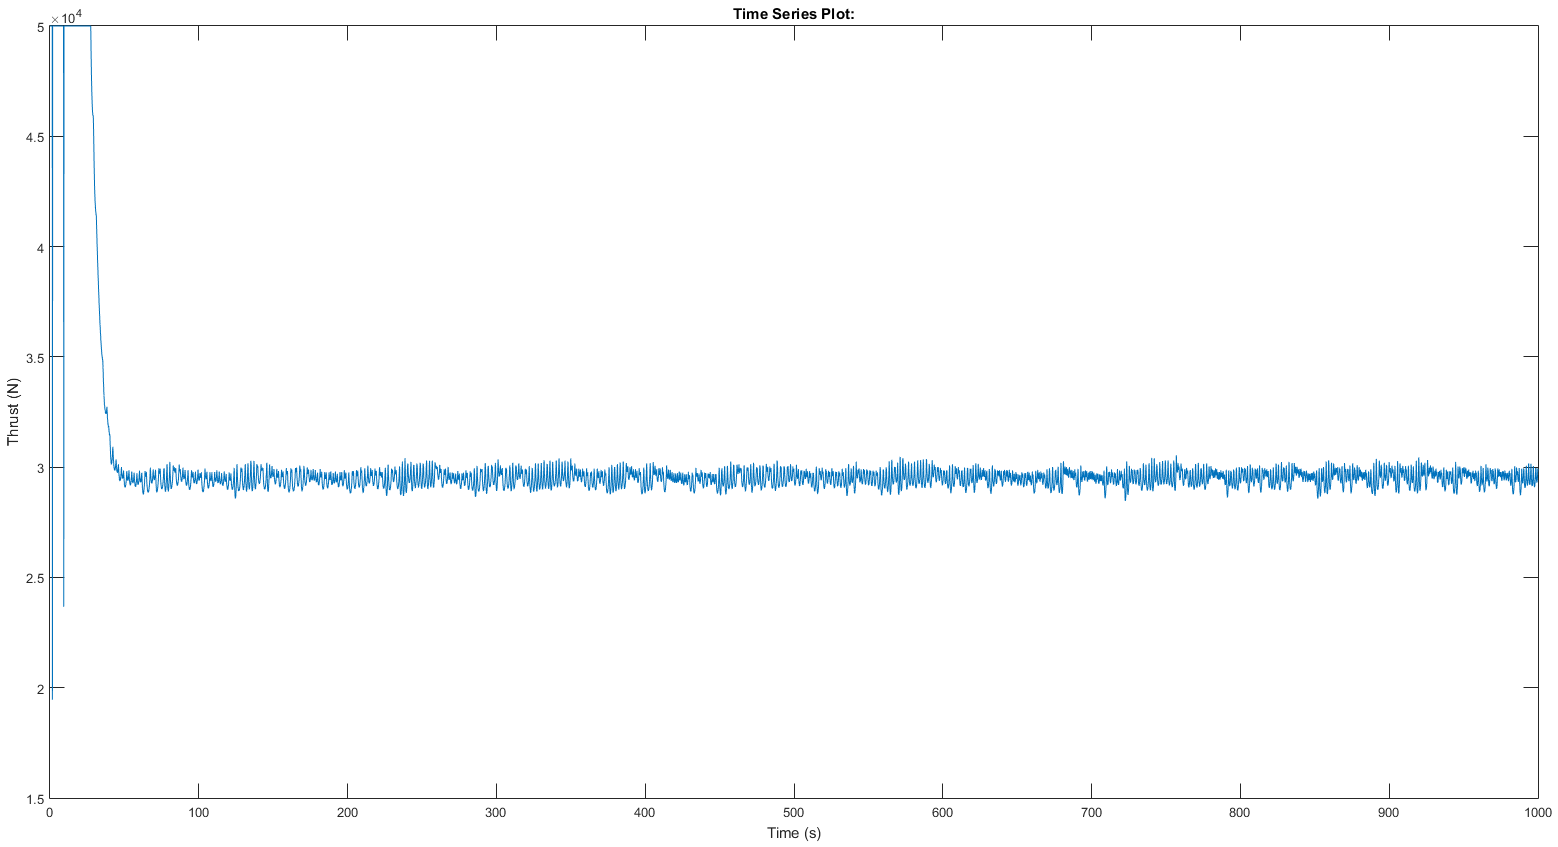
\includegraphics[width=\textwidth]{Figures/Results/thrust_check.PNG}
\end{minipage}
\caption[AoA and thrust validation]{Angle of Attack (degrees) and thrust (Newton) of the controlled aircraft}
\end{figure}

This simulation, made over 800 seconds, shows clearly that the angle oscillates around a $6^o$ degree angle of attack, with an amplitude of around $0.4^o$ degrees. As for the thrust, it also oscillates around $30000N$ with an amplitude of $2000N$. These values correspond to the theoretical values in table \ref{tab:cruise_cond} for $\alpha=6^o$, indicating that not only the modelled plane is well behaved, but also that the coefficient neural networks are able to simulate an accurate model of the aerodynamic coefficient's variation.


%%%%%%%%%%%%%%%%%%%%%%%%%%%%%%%%%%%%%%%%%%%%%%%%%%%%%%%%%%%%%%%%%%%%%%%%
\section{Feedback linearisation controller}
\label{section:results/fl_contro}

Once the model has been tested and validated, the described nonlinear inversion controller can now be tested. Reference tracking will firstly be observed with simple constant reference values, without any guidance control law. Reiterating the example from the previous section in cruise conditions for $V_a^d=200 ms^{-1}$, $\gamma^d = 0^o$ and $\psi^d = 0^o$ comes that
\begin{figure}[h]
\centering
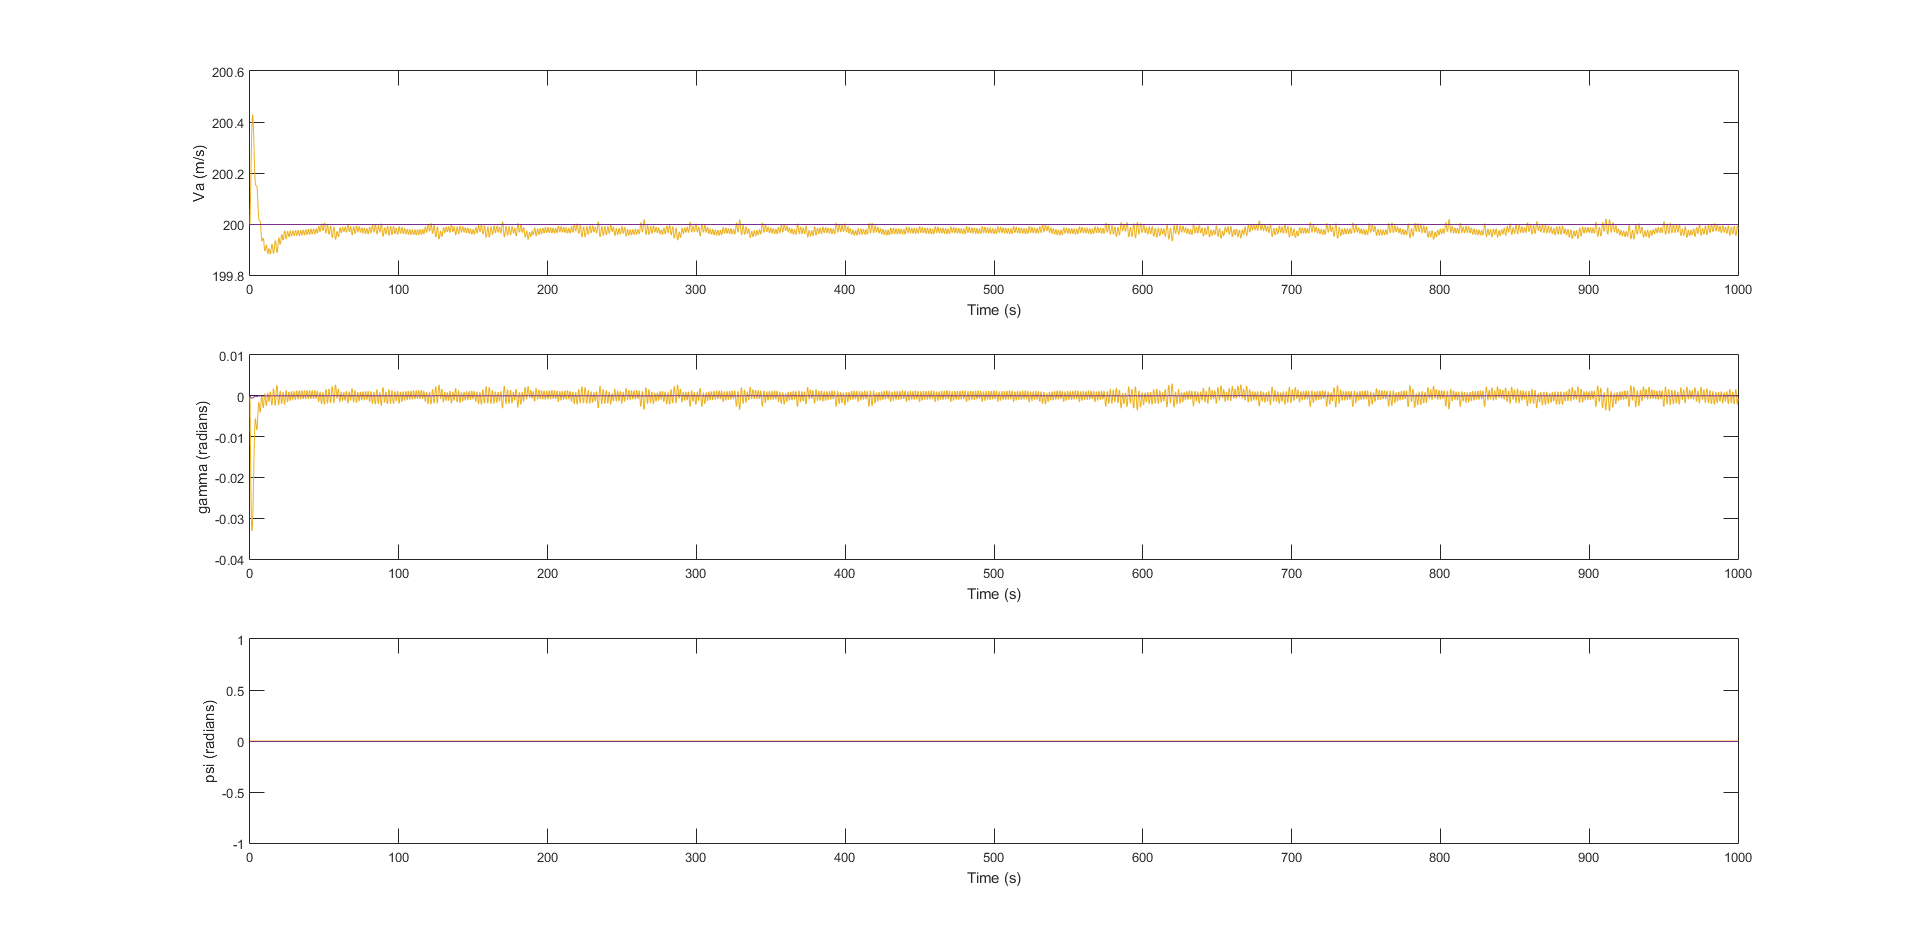
\includegraphics[width=\textwidth]{Figures/Results/nli_test_const.png}
\caption[Constant reference following of feedback linearisation controller]{Reference (blue) following over $1000s$ of simulation time for $V_a^d=200 ms^{-1}$, $\psi^d = 0^o$ and $\gamma^d = 0^o$ respectively and measured values (yellow)}
\label{fig:const_ref}
\end{figure}

As seen in the figure \ref{fig:const_ref} the reference is followed with minimal osculations for the three variables, although with the presence of some steady state error in the case of the airspeed $V_a$. To be able to follow trajectories however, a good control of the aircraft's heading will be necessary. Proposing this time the following variation in $\psi^d$
\begin{equation}
\psi^d = \begin{cases}
0^o & t < 100\\
90^o & 100 \leq t < 500\\
0^o & t > 500 \\
\end{cases}
\end{equation}


\section{Disturbances and Errors}
\label{section:results/disturbances_errors}


\section{Neural Network}
\label{section:results/NN}

\section{Guidance controller}
\label{section:results/guidance_control}


